\documentclass[11pt,a4paper,oneside]{article}
\usepackage{preamble}
\title{The Poset of Mesh Patterns}

\begin{document}
	\maketitle

\section{Introduction}
Mesh patterns are a generalisation of permutations and have been studied extensively in recent years, see e.g.,~\cite{CTU15,JKR15}.
A natural definition of when one mesh patterns occurs in another mesh patterns was given in~\cite{TU17}.
This allows us to generalise the classical permutation poset to a poset of mesh patterns, where
$(\sigma,S)\le(\pi,P)$ if there is an occurrence of $(\sigma,S)$ in~$(\pi,P)$.

The poset of permutations has received a lot of attention in recent years, but due to its
complicated structure a full understanding of the poset has proven elusive,
see \cite{Smith14,Smith15}. The poset of mesh patterns, which we define
here, contains the poset of permutations as an induced subposet. By studying this poset we
hope to see if the two posets posses a similar structure, so that a understanding of one
may lead to results on the other.

There are many open questions relating to mesh patterns, for example two mesh patterns
are \emph{coincident} if their avoidance classes are exactly the same. A full classification
of such coincidences has proven difficult to obtain, see \cite{CTU15}. By looking at
the structure of the poset,
we hope for a better understanding of mesh patterns and their properties,
such as coincidences.

In \cref{sec:PosMP} we introduce the poset of mesh patterns and related definitions,
including a brief overview of poset topology. In \cref{sec:MF} we prove some results
on the M\"obius function of the poset of mesh patterns. In \cref{sec:purity} we give
a characterisation of the non-pure intervals of the mesh pattern poset.
In \cref{sec:topology} we give some results on the topology of the mesh pattern poset.



\section{The Poset of Mesh Patterns}\label{sec:PosMP}
Mesh patterns were first introduced in \cite{Bra11} and
are a generalisation of permutations. Given a permutation
$\pi=\pi_1\pi_2\ldots\pi_n$ we can plot $\pi$ on an $n\times n$ grid,
where we place a dot at coordinates $(i,\pi_i)$, for all $1\le i\le n$.
A mesh pattern is then obtained by shading boxes of this grid, so a mesh
pattern takes the from $p=(\cl{p},\sh{p})$, where $\cl{p}$ is a permutation
and $\sh{p}$ is a set of coordinates recording the shaded boxes, which are indexed
by their south west corner. For ease of notation we sometimes denote the mesh
pattern $\cl{p}^{\sh{p}}$. We let $|\cl{p}|$ represent the length of $\cl{p}$
and $|\sh{p}|$ the size of $\sh{p}$, and define the \emph{length} of $p$ as $|\cl{p}|$.
For example, the mesh pattern $(132,\{(0,0),(0,1),(2,2)\})$,
or equivalently $132^{(0,0),(0,1),(2,2)}$, has the form:
\begin{center}
\patt{0.5}{3}{1,3,2}[0/1,0/0,2/2][][][][][4]
\end{center}

To define when a mesh pattern occurs within another mesh pattern, first we need to
recall two other well-known definitions of occurrence. A permutation $\sigma$
\emph{occurs} in a permutation $\pi$ if there is a subsequence, $\eta$, of $\pi$ whose letters
appear in the same relative order of size as the letters of $\sigma$. The subsequence
$\eta$ is called an \emph{occurrence}.

Consider a mesh pattern $(\sigma,S)$ and an occurrence $\eta$ of $\sigma$ in $\pi$, in the
classical permutation pattern sense. Each box $(i,j)$ of $(\sigma,S)$ corresponds to an
area $R_{\eta}(i,j)$ in the plot of $\pi$, which is the area bounded by the points in $\pi$
which in $\eta$ correspond to the letters $\sigma_i,\sigma_{i+1},j,j+1$ of $\sigma$.
We say that $\eta$ is an occurrence of the mesh pattern $(\sigma,S)$ in the permutation~$\pi$
if there is no point in any of the areas $R_{\eta}(i,j)$ for any shaded box~$(i,j)\in S$.

Using these definitions of occurrences we can recall a concept of mesh
pattern containment in another mesh pattern introduced in \cite{TU17}.
An example of which is given in \cref{fig:occEx}.

\begin{defn}[\cite{TU17}]\label{defn:meshOcc}
An occurrence of a mesh pattern $(\sigma,S)$ in another mesh
pattern $(\pi,P)$ is an occurrence~$\eta$ of~$(\sigma,S)$ in $\pi$, where for any $(i,j)\in S$
every box in $R_\eta(i,j)$ is shaded in $(\pi,P)$.
\end{defn}

\begin{figure}\centering
\begin{subfigure}[b]{0.3\textwidth}
\centering\patt{0.75}{2}{1,2}[0/1,0/2,2/2][][][][]
\caption{}\label{subfiga}\end{subfigure}
\begin{subfigure}[b]{0.3\textwidth}
\centering\patt{0.75}{3}{1,2,3}[0/0,0/2,0/3,1/3,1/1,1/2,2/1,2/2,3/3][][][][]
\caption{}\label{subfigb}\end{subfigure}
\begin{subfigure}[b]{0.3\textwidth}\centering
\colpatt{0.75}{3}{1,2,3}[0/0,0/2,0/3,1/3,1/1,1/2,2/1,2/2,3/3][2/2,3/3][3/3,0/2,0/3,1/3,1/2]
\caption{}\label{subfigc}\end{subfigure}
\caption{A pair of mesh patterns (a) and (b), with (c) showing an occurrence of (a) in~(b).
 Also note (b) does not contain $12^{(0,0),(1,1),(2,2)}$.}\label{fig:occEx}
\end{figure}

The classical permutation poset $\mathcal{P}$ is defined as the poset of all permutation,
with $\sigma\le_\mathcal{P}\pi$ if and only if $\sigma$ occurs in $\pi$. Using \cref{defn:meshOcc}
we can similarly define the poset of mesh patterns $\mathcal{M}$ as the poset of all mesh patterns,
with $m\le_\mathcal{M} p$ if $m$ occurs in $p$. Note we drop the subscripts from $\le$ when it is clear
which partial order is being considered. An \emph{interval} $[\alpha,\beta]$ of a poset is defined as subposet induced by the set
$\{\kappa\,|\,\alpha\le\kappa\le\beta\}$. See \cref{fig:intEx} for an example of an interval of $\mathcal{M}$.

\begin{figure}\centering
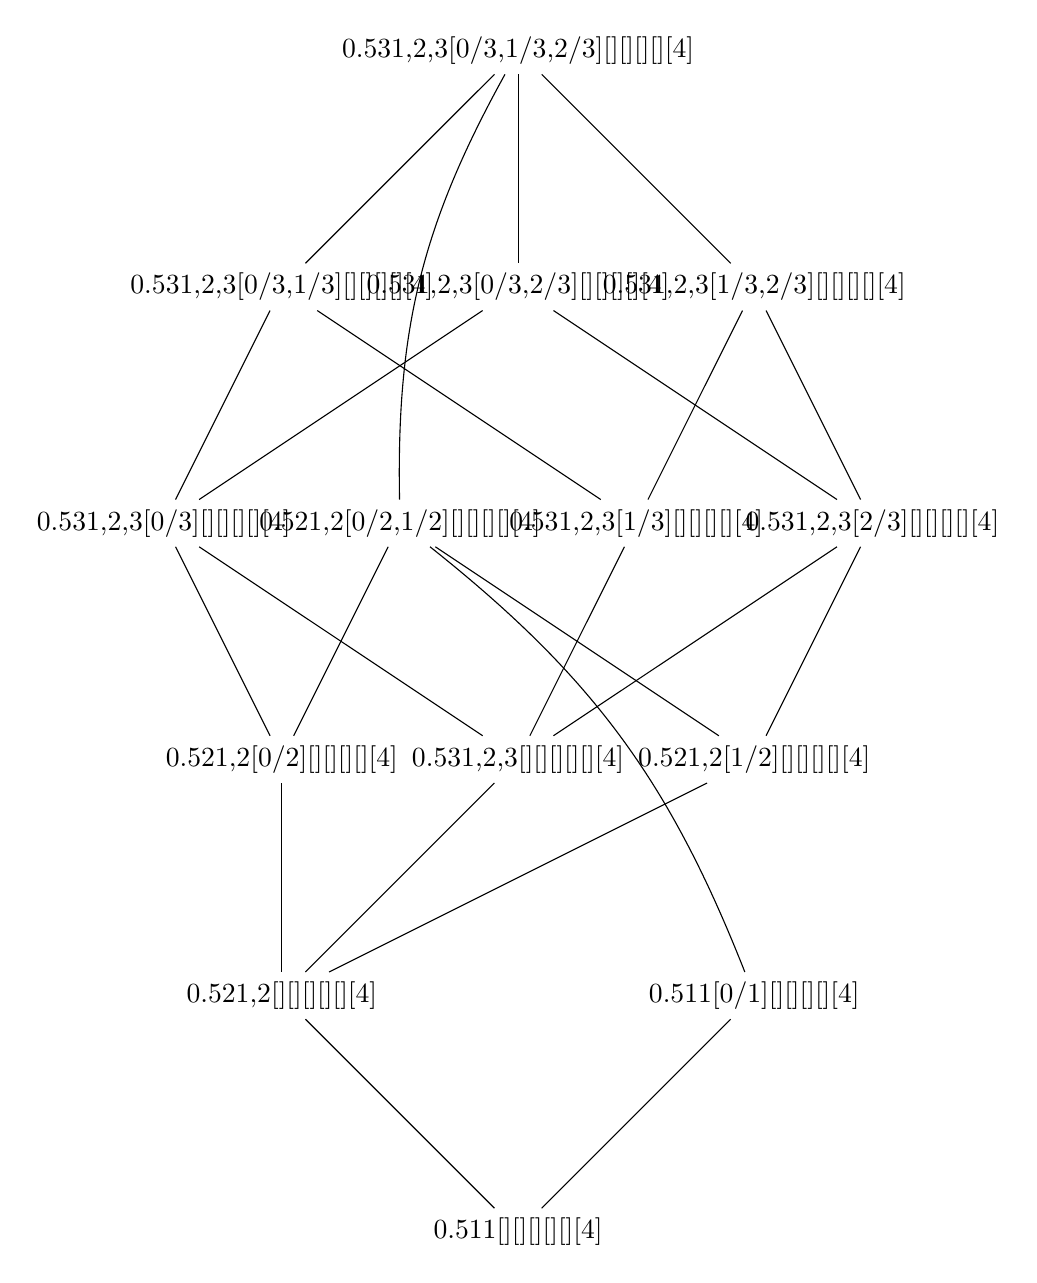
\begin{tikzpicture}
\def\y{3}
\def\x{3}
\def\s{0.5}
\node (123-123) at (0*\x,5*\y){\patt{\s}{3}{1,2,3}[0/3,1/3,2/3][][][][][4]};
\node (123-12) at (-1*\x,4*\y){\patt{\s}{3}{1,2,3}[0/3,1/3][][][][][4]};
\node (123-13) at (0*\x,4*\y){\patt{\s}{3}{1,2,3}[0/3,2/3][][][][][4]};
\node (123-23) at (1*\x,4*\y){\patt{\s}{3}{1,2,3}[1/3,2/3][][][][][4]};
\node (123-1) at (-1.5*\x,3*\y){\patt{\s}{3}{1,2,3}[0/3][][][][][4]};
\node (12-12) at (-0.5*\x,3*\y){\patt{\s}{2}{1,2}[0/2,1/2][][][][][4]};
\node (123-2) at (0.5*\x,3*\y){\patt{\s}{3}{1,2,3}[1/3][][][][][4]};
\node (123-3) at (1.5*\x,3*\y){\patt{\s}{3}{1,2,3}[2/3][][][][][4]};
\node (12-1) at (-1*\x,2*\y){\patt{\s}{2}{1,2}[0/2][][][][][4]};
\node (123-0) at (0*\x,2*\y){\patt{\s}{3}{1,2,3}[][][][][][4]};
\node (12-2) at (1*\x,2*\y){\patt{\s}{2}{1,2}[1/2][][][][][4]};
\node (12-0) at (-1*\x,1*\y){\patt{\s}{2}{1,2}[][][][][][4]};
\node (1-1) at (1*\x,1*\y){\patt{\s}{1}{1}[0/1][][][][][4]};
\node (1-0) at (0*\x,0*\y){\patt{\s}{1}{1}[][][][][][4]};
\draw (123-123) -- (123-12);\draw (123-123) -- (123-13);\draw (123-123) -- (123-23);
\draw[-] (123-123) to [bend right=15] (12-12);\draw[-] (12-12) to [bend left=15] (1-1);
\draw (123-12) -- (123-1);\draw (123-12) -- (123-2);
\draw (123-13) -- (123-1);\draw (123-13) -- (123-3);
\draw (123-23) -- (123-2);\draw (123-23) -- (123-3);
\draw (123-1) -- (123-0);\draw (123-1) -- (12-1);
\draw (123-2) -- (123-0);
\draw (123-3) -- (123-0);\draw (123-3) -- (12-2);
\draw (12-12) -- (12-1);\draw (12-12) -- (12-2);
\draw (12-1) -- (12-0);\draw (12-2) -- (12-0);
\draw (123-0) -- (12-0);\draw (12-0) -- (1-0);
\draw (1-1) -- (1-0);
\end{tikzpicture}
\caption{The interval $[1^\emptyset,123^{(0,3),(1,3),(2,3)}]$ of $\mathcal{M}$.}\label{fig:intEx}
\end{figure}

The first result on the mesh pattern poset is that there are infinitely many maximal
elements, which shows a significant difference to the permutation poset, where there are no maximal elements.

\begin{lem}\label{lem:max}
The poset of mesh pattern contains infinitely many maximal elements, which are the mesh
patterns in which all boxes are shaded.
\end{lem}

\begin{proof}
This follows from the easily proven fact that a fully shaded mesh patterns only
occurs in itself, and no other mesh patterns.
\end{proof}


\subsection{Poset Topology}
In this subsection we briefly introduce some poset topology and, refer the reader to \cite{Wac07}
for a comprehensive overview of the topic, including any definitions we omit here.

The \emph{M\"obius function} on an interval $[\alpha,\beta]$ of a poset is defined by:
$\mu(a,a)=1$, for all $a$, $\mu(a,b)=0$ if $a\not\le b$, and $$\mu(a,b)=-\sum_{c\in[a,b)}\mu(a,c).$$
We refer to $\mu(a,b)$ as the M\"obius function of $[a,b]$. See \cref{fig:1-123} for an example.

In a poset we say that $\alpha$ \emph{covers} $\beta$, denoted $\alpha\gtrdot\beta$, if $\alpha>\beta$
and there is no $\kappa$ such that $\alpha>\kappa>\beta$. A \emph{chain} of length $k$ in a poset is
a totally ordered subset $c_1<c_2<\cdots<c_{k+1}$, and the chain is maximal if $c_i\lessdot c_{i+1}$,
for all $1\le i \le k$. A poset is \emph{pure} (also known as \emph{ranked} or \emph{graded}) if all
maximal chains have the same length. The \emph{dimension} of a poset $P$, denoted $\dim P$, is the
length of the longest maximal chain. For example, the interval in \cref{fig:intEx} is nonpure because
there is one maximal chain of length $3$ ($\pattin{1}{1}{}\lessdot\pattin{1}{1}{0/1}\lessdot
\pattin{2}{1,2}{0/2,1/2}\lessdot\pattin{3}{1,2,3}{0/3,1/3,2/3}$) and all other maximal chains have
length $5$, so the dimension is $5$.

The \emph{interior} of an interval $[\alpha,\beta]$ is obtained by removing $\alpha$ and $\beta$,
and is denoted $(\alpha,\beta)$. The \emph{order complex} of an interval $[\alpha,\beta]$, denoted
$\Delta(\alpha,\beta)$ is the simplicial complex whose faces are the chains of $(\alpha,\beta)$.
When we refer to the topology of an interval we mean the topology of the order complex of the interval.

The \emph{reduced Euler characteristic} $\tilde{\chi}$ of a simplicial complex is a topological invariant
which counts the number ``holes'' in the complex. The Philip Hall Theorem~\cite{Hall36} implies that
$\mu(\sigma,\pi)=\tilde{\chi}(\Delta(\sigma,\pi)$. Therefore, by studying the topology of the order
complex of a poset we can derive results on the M\"obius function.

A poset is \emph{shellable} if we can order the maximal chains of the interior $F_1,\ldots,F_t$
such that the induced subposet $\left(\cup_{i=1}^{k-1}F_i\right)\cap F_k$ is pure and
$(\dim F_k)$-dimensional, for all $k=2,\ldots,t$. Being shellable implies other properties
on the topology, such as having the homotopy type of a wedge of spheres.

An interval is \emph{disconnected} if the interior can be split into two disjoint sets, called
\emph{components}, which are pairwise incomparable, that is, $a\not\le b$ and $b\not\le a$ if
$a$ and $b$ belong to different sets. We call a component \emph{non-trivial} if it contains more than one point
and we say an interval is \emph{strongly disconnected} if at least two components are nontrivial.

We can use disconnectivity as a test for shellability using the following results.

\begin{lem}\label{lem:strongdis}
If an interval is strongly disconnected, then it is not shellable.
\begin{proof}
For any ordering of the maximal chains, the intersection of the first chain of the second non-trivial
component with the preceding chains is the empty set, which has dimension $-1$, and as the component is
non-trivial the chain must have dimension at least $1$. Therefore, the shellable conditions cannot be
satisfied by any ordering.
\end{proof}
\end{lem}

Since every subinterval of a shellable interval is shellable, \cite[Corollary 3.1.9]{Wac07},
we obtain the following:

\begin{cor}
An interval which contains a strongly disconnected interval is not shellable.
\end{cor}

Finally, we present a useful result known as the Quillen fiber lemma~\cite{Quillen78}. Two simplicial
complexes are homotopy equivalent  if one can be obtained by deforming the other but
not breaking or creating any new ``holes", so their Euler
characteristic is the same. Therefore, if two posets are homotopy equivalent their
M\"obius functions are equal. A simplicial complex is \emph{contractable} if it contains
no holes and given a poset $P$, with $p \in P$ define the upper ideal $P_{\ge p}=\{q\in P\,|\,q\ge p\}$.

\begin{prop}\label{thm:Quil}(Quillen Fiber Lemma)
Let $\phi:P\rightarrow Q$ be an order-preserving map between posets such that for any
$x\in Q$ the complex $\Delta(\phi^{-1}(Q_{\ge x}))$ is contractible.
Then $P$ and $Q$ are homotopy equivalent.
\end{prop}

In the subsequent sections we give some results on the M\"obius function and topology of
the poset of mesh patterns.

\section{M\"obius Function}\label{sec:MF}
In this section we present some results on the M\"obius function of the mesh pattern poset.
We begin with some simple results: on mesh patterns with the same underlying permutations;
the mesh patterns with no points $\epsilon^\emptyset$ and $\epsilon^{(0,0)}$;
and mesh patterns with no shaded boxes.
Throughout, the remainder of the paper we assume that $m$ and $p$ are
mesh patterns.

\begin{lem}
If $\cl{m}=\cl{p}$, then $[m,p]$ is isomorphic to the boolean lattice
$B_{|\sh{p}|-|\sh{m}|}$, which implies $\mu(m,p)=(-1)^{|\sh{p}|-|\sh{m}|}$ and
$[m,p]$ is shellable.
\begin{proof}
We cannot remove any points from $p$, but we can
unshade any boxes from $\sh{p}\setminus\sh{s}$ in any order.
\end{proof}
\end{lem}

\begin{lem}
Consider $A\in\{\emptyset,(0,0)\}$, then:
$$\mu(\epsilon^{A},p)=\begin{cases}
1,&\mbox{ if }p=\epsilon^A \\
-1,&\mbox{ if }A=\emptyset\,\,\&\,\,|\cl{p}|+|\sh{p}|=1\\
0,&\mbox{ otherwise}
\end{cases}.$$
\begin{proof}
The first two cases are trivial. The
mesh pattern $\epsilon^{(0,0)}$ is not contained in any larger mesh patterns, so
the M\"obius function is always $0$. If $|\cl{p}|+|\sh{p}|>1$, then
$(\epsilon^\emptyset,p)$ contains a unique minimal element $1^\emptyset$, so
$\mu(\epsilon^\emptyset,p)=0$.
\end{proof}
\end{lem}

\begin{lem}
If $\sh{s}=\sh{p}=\emptyset$, then $[s,p]$ is isomorphic to
$[\cl{s},\cl{p}]$ in $\mathcal{P}$, so $$\muM(s,p)=\muP(\cl{s},\cl{p}).$$
\end{lem}

The M\"obius function of the classical permutation poset is known to be
unbounded \cite{Smith13}. So we get the following corollary:

\begin{cor}
The M\"obius function is unbounded on $\mathcal{M}$.
\end{cor}

We can also show that the M\"obius function is unbounded if we include shadings.
We do this by mapping to the poset of words with subword order.
This is the poset made up of all words and $u\le w$ if there is a subword of $w$
that equals $u$.
A \emph{descent} in a permutation $\pi=\pi_1,\pi_2,\ldots,\pi_n$ is a pair of
letters $\pi_i,\pi_{i+1}$ with $\pi_{i}>\pi_{i+1}$. We call $\pi_{i+1}$ the \emph{descent bottom}.
An \emph{adjacency} in a permutation is a consecutive sequence of $t>1$ consecutively valued letters,
such as $23$ or $654$ in $236541$.

\begin{lem}\label{lem:mobUn}
Let $m$ be a mesh pattern with exactly one descent, where the descent bottom is
$1$, and all boxes south west of which are shaded, then
\[
\mu(21^{(0,0),(1,0)},m)=\begin{cases}
(-1)^{|m|}\lfloor\frac{n}{2}\rfloor,&\text{ if } \cl{m} \text{ has no adjacencies}\\
1,&\substack{ \text{ if } \cl{m} \text{ has exactly adjacency and it is before the descent with length }2}\\
0, &\text{ otherwise}
\end{cases}
\]
Moreover, $[21^{(0,0),(1,0)},m]$ is shellable.
\begin{proof}
Note that every mesh pattern in $I=[21^{(0,0),(1,0)},m]$ satisfies the same
descent conditions as $m$. So each mesh pattern is uniquely determined by
which letters are before $1$, because we put those letters in increasing order,
then $1$, then the remaining letters in increasing order and finally shade
everything south west of $1$.

So define a bijection $f$ from $I$ to
the poset of words with subword order, where the $i-1$'th letter of $f(p)$ is $0$
if $i$ is before $1$ in $\cl{p}$ and $1$ otherwise, for all
$1<i\le n$, so $f(21^{(0,0),(1,0)})=0$.
Because the mesh patterns are uniquely determined by the letters before $1$,
it is straightforward to see this is a bijection and to
check that it is order preserving. So $I$ is isomorphic to an interval of the
poset of words with subword order.

 It was shown in \cite{Bjo90} that these
intervals are shellable and the M\"obius function equals the number of normal
occurrences, where an occurrence is \emph{normal} if in any run of equal elements every
non-initial letter is part of the occurrence. In our bijection a run in the word
is mapped to an adjacency in the permutation. Moreover, in every occurrence of
$21^{(0,0),(1,0)}$ in $m$ the $1$ of $21$ must occur as the $1$ in $m$. So
all that remains is to place the $2$ somewhere and for the occurrence to be normal
every non-initial letter of an adjacency must be in the occurrence, this imples the result.
\end{proof}
\end{lem}

We can also see that the M\"obius function on $\mathcal{M}$ is not bounded by
the classical permutation poset, that is, it is not true that $\muM(m,p)\le
\muP(\cl{m},\cl{p})$. A simple counterexample is the interval
$[1^{(0,1)},123^{(0,2),(0,3),(1,2),(1,3)}]$, this has M\"obius function $1$,
however $\muP(1,123)=0$, see \cref{fig:1-123}.

\begin{figure}\centering
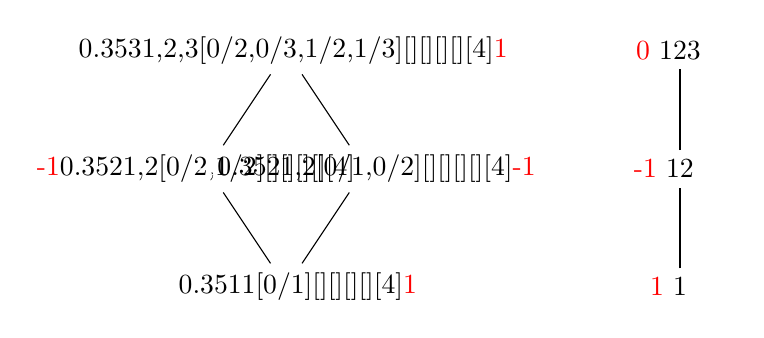
\begin{tikzpicture}
\def\s{0.35}
\node (123) at (0,3){\textcolor{white}{1}\patt{\s}{3}{1,2,3}[0/2,0/3,1/2,1/3][][][][][4]\textcolor{red}{1}};
\node (12a) at (-1,1.5){\textcolor{red}{-1}\patt{\s}{2}{1,2}[0/2,1/2][][][][][4]\textcolor{white}{-1}};
\node (12b) at (1,1.5){\textcolor{white}{-1}\patt{\s}{2}{1,2}[0/1,0/2][][][][][4]\textcolor{red}{-1}};
\node (1) at (0,0){\textcolor{white}{-1}\patt{\s}{1}{1}[0/1][][][][][4]\textcolor{red}{1}};
\draw (1) -- (12a) -- (123) -- (12b) -- (1);
\node (123) at (5,3){\textcolor{red}{0} $123$ \textcolor{white}{0}};
\node (12) at (5,1.5){\textcolor{red}{-1} $12$ \textcolor{white}{-1}};
\node (1) at (5,0){\textcolor{red}{1} $1$ \textcolor{white}{1}};
\draw (1) -- (12) -- (123);
\end{tikzpicture}
\caption{The interval $[1^{(0,1)},123^{(0,2),(0,3),(1,2),(1,3)}]$
(left) in $\mathcal{M}$ and $[1,123]$ (right) in $\mathcal{P}$,
with the M\"obius function in red.}\label{fig:1-123}
\end{figure}

If we consider intervals where the bottom mesh pattern has no shadings, then we
get the following result:
\begin{lem}\label{lem:mu0}
Consider the interval $[m,p]$ in $\mathcal{M}$. If $\sh{m}=\emptyset\not=\sh{p}$
and there is no $s\in(m,p)$ with $\cl{s}=\cl{m}$, then $\mu(m,p)=0$.
\begin{proof}
Define a map $f(x)=\cl{x}^\emptyset$, for any $x\in(m,p)$, and let $A:=f((m,p))$, then $A=(\cl{m}^\emptyset,\cl{p}^{\emptyset}]$.
So  $A$ is contractible, because it has the
unique maximal element $\cl{p}^\emptyset$, so $\mu(A)=0$. Moreover, $f^{-1}(A_{\ge y})$
equals $[y,p)$, for all $y\in A$, which is contractible. Therefore, $(m,p)$ is homotopically equivalent
to $A$ by the Quillen Fiber Lemma, which implies $\mu(m,p)=0$.
\end{proof}
\end{lem}

We can combine Lemma~\ref{lem:mu0} with the following result to see that the
M\"obius function is almost always zero on the interval $[1^\emptyset,p]$.

\begin{lem}
As $n$ tends to infinity the proportion of permutations of length $n$ that contain one of
$\{1^{(0,0)},1^{(1,0)},1^{(0,1)},1^{(1,1)}\}$ approaches $0$.
\begin{proof}
Let $P(n,i)$ be the probability that the letter $i$ is an occurrence of
$1^{(0,0)}$ in a length $n$ mesh pattern. And let $P(n)$ be the probability
that a length $n$ mesh pattern contains $1^{(0,0)}$.

The probability that $i$ is an occurrence of $1^{(0,0)}$ is given by selecting
the location $k$ of $i$, each has probability $\frac{1}{n}$, and then we require
that all boxes south west of $i$ are filled, of which there are $2^{ik}$. Note
that this over estimates the probability, because it is possible that there is a
point south west of $i$, which would imply $i$ is not an occurrence of
$1^{(0,0)}$, however this argument still counts them. We can formulate this as:
\begin{align*}
P(n,i)&\le\sum_{k=1}^{n+1-i}\frac{1}{n}\left(\frac{1}{2^i}\right)^k
=\frac{1}{n}\left(\frac{2^{-i(n+2-i)}}{2^{-i}-1}-1\right)
=\frac{1}{n2^i}\left(\frac{1-2^{-i(n+1-i)}}{1-2^{-i}}\right)
\le\frac{2}{n2^i}
\end{align*}

To compute the probability that a length $n$ permutation contains $1^{(0,0)}$ we
can sum over all letters $i$ and test if $i$ is an occurrence of $1^{(0,0)}$.
Note again this is an over estimate because if a permutation contains multiple
occurrences of $1^{(0,0)}$ it counts that permutation more than once.

$$
P(n)\le\sum_{i=1}^{n}P(n,i)\le\sum_{i=1}^{n}\frac{2}{n2^i}
=\frac{2}{n}\left(\frac{\left(\frac{1}{2}\right)^{n+1}-1}{\frac{1}{2}-1}-1\right)
\le\frac{2}{n}
$$

We can repeat this calculation for the other three shadings of $1$ so we get
that $P(n)\le \frac{8}{n}\rightarrow 0$.
\end{proof}
\end{lem}
\begin{cor}
As $n$ tends to infinity the proportion of mesh patterns $p$ of length n such
that $\mu(1^\emptyset,p)=0$ approaches $1$.
\end{cor}


In the classical case it is true that given a permutation $\sigma$ the
probability a permutation of length $n$ contains $\sigma$ tends to $1$ as $n$
tends to infinity, this follows from the Marcus-Tardos Theorem \cite{MT04}. By
the above result we can see the same is not true in the mesh pattern case. In
fact we conjecture the opposite is true:
\begin{conj}
Given a mesh pattern $m$, the probability that a random mesh pattern of length
$n$ contains $m$ tends to $0$ as $n$ tends to infinity.
\end{conj}




\section{Purity}\label{sec:purity}
Recall that a poset is pure if all the maximal chains have the same length, and as we
can see from \cref{fig:intEx} the mesh pattern poset is non-pure. In this section we classify
which intervals~$[1^\emptyset,m]$ are non-pure. First we consider the length of the longest maximal chain in
any interval~$[1^\emptyset,m]$, that is, the dimension of $[1^\emptyset,m]$.

\begin{lem}
For any mesh pattern $m$, we have $\dim(1^\emptyset,m)=|\cl{m}|+|\sh{m}|$.
\begin{proof}
We can create a chain from $m$ to $1^\emptyset$ by deshading all boxes, in any order,
and then deleting all but one point, in any order. The length of this chain is $|\cl{m}|+|\sh{m}|$.
Moreover, to create a smaller element at least one shading or point must be removed,
 so we cannot create a chain of length greater than $|\cl{m}|+|\sh{m}|$.
\end{proof}
\end{lem}

So we define the \emph{dimension} of a mesh pattern as $\dim(m)=|\cl{m}|+|\sh{m}|$ and we say an
edge $m\lessdot p$ is \emph{impure} if $\dim(p)-\dim(m)>1$.
Next we give a classification of impure edges.

 Let $m-x$ be the mesh pattern obtained by deleting the
point $x$ and let $m\setminus x$ be the occurrence of $m-x$ in $m$ that does not
use the point $x$. An occurrence $\eta$ of $m$ in $p$ \emph{uses the shaded box $(a,b)\in\sh{p}$}
if $(a,b)\in R_\eta(i,j)$ for some shaded box $(i,j)\in\sh{m}$. We say that
deleting a point $x$ \emph{merges shadings} if
there is a shaded box in $m-x$ that corresponds to more than one shaded box in
$m\setminus x$, see \cref{fig:impEx}.

\begin{lem}\label{lem:impureEdge}
Two mesh patterns $m<p$ form an impure edge if and only if all occurrences of $m$ in
$p$ use all shaded boxes of $p$ and are obtained by deleting a point that merges
shadings.
\end{lem}

\begin{proof}
First we show the backwards direction. Because $m$ is obtained by deleting a
point that merges shadings, $m$ must have one less point and at least one less
shading so $\dim(p)-\dim(m)\ge2$. So it suffices to show that there is no $z$ such
that $m<z<p$. Suppose such a $z$ exists, then if $z$ is obtained by deshading a
box in $p$ it can no longer contain $m$ because all occurrences of $m$ in $p$
use all shaded areas of $p$. If $z$ is obtained by deleting a point, then that
cannot remove shadings, only merge shadings, otherwise it wouldn't contain $m$,
and it implies $\cl{m}=\cl{z}$. Moreover, if $m<z$ then we can deshade some boxes
of $z$ to get $m$ which implies there is an occurrence of $m$ in $p$ that
doesn't use all the shaded boxes of $p$.

Now consider the forwards direction. Suppose $m\lessdot p$ is impure. So
$\dim(p)-\dim(m)\ge2$, which implies $m$ is obtained by deleting a single point
which merges shadings but does not delete shadings, because any other
combination of deleting points and deshading can be done in successive steps.
Furthermore, this must be true for any point that can be deleted to get $m$,
that is, for all occurrences of $m$ in $p$. Moreover, if there is an occurrence
that doesn't use all the shaded boxes of $p$, we can deshade the box it doesn't
use and get an element that lies between $m$ and $p$.
\end{proof}

\begin{figure}\centering
\begin{subfigure}[b]{0.3\textwidth}
\centering\colpatt{0.5}{2}{1,2}[0/2,1/2][2/2][0/2,1/2]
\caption*{$a=12^{(0,2),(1,2)}$}\label{subfig:a}\end{subfigure}
\begin{subfigure}[b]{0.3\textwidth}
\centering\colpatt{0.5}{3}{1,2,3}[1/3,2/3][1/1,3/3][1/3,2/3]
\caption*{$b=123^{(1,3),(2,3)}$}\label{subfig:b}\end{subfigure}
\caption{Two mesh patterns with a point $x$ in black which merges shadings and the occurrences
$a\setminus x$ and $b\setminus x$ in red. By \cref{lem:impureEdge} $a-x\lessdot a$ is impure,
but $b-x<b$ is not an impure edge because there is a second occurrence of $b-x$ in $b$, using points $23$,
that does not use all shaded boxes in $b$.}\label{fig:impEx}
\end{figure}

\begin{lem}\label{lem:topImpure}
If there is an impure edge in $[1^\emptyset,m]$, then there is an impure edge
$a\lessdot b$ where $\cl{m}=\cl{b}$.
\begin{proof}
If $x\lessdot y$ is an impure edge in $[1^\emptyset,m]$, then let $b$ be a mesh
pattern obtained by adding points to $y$ so $\cl{b} = \cl{m}$. Pick
an occurrence of $x$ in $y$ and add the points to $x$ in the positions induced by
how they are added to $y$ and the occurrence, call this $a$. The points added
will not have any shadings in the four boxes touching it, therefore no point
touching a shading in $a$ can embed in a new point of $b$. Moreover, the set of
occurrences of $a$ in $b$ is a subset of $x$ in $y$, after adding the new points
to each. These two conditions imply that every occurrence of $x$ in $y$ uses
all the shadings of $y$, this is also true for every occurrence of $a$ in $b$.
Therefore, the result follows by Lemma~\ref{lem:impureEdge}.
\end{proof}
\end{lem}

\begin{prop}
The interval $[1^\emptyset,m]$ is non-pure if and
only if there exists a point $p$ in $m$ such that $m-p$ merges shadings and
there is no other occurrence of $m-p$ in $m$ which uses a subset of shadings of
used by $m\setminus p$.
\begin{proof}
First we show the backwards direction. Let $x$  be the mesh pattern obtained by
inserting $p$ back into $m-p$, and $\eta$ the corresponding occurrence of $m-p$
in $x$. Note that it is not always true that $x=m$ because some shadings
of $m$ are lost when deleting $p$. We claim that $m-p\lessdot x$ is an impure
edge. This follows by Lemma~\ref{lem:impureEdge} because $\eta$ uses all the
shaded boxes in $x$ and there is no subshading occurrence.

To see the other direction suppose there is an impure edge in $[1^{\emptyset},m]$. By
Lemma~\ref{lem:topImpure} there is an impure edge $a\lessdot b$ where
$\cl{b}=\cl{m}$. If $m$ is impure then it must remove both a point and a shading,
so it must merge shadings by deleting some point $p$ and there is no element
between them so there can be no subshading of $b$ that contains $a$.
\end{proof}
\end{prop}

\begin{cor}
There is an impure edge in the interval $[m,p]$ if and only if there exists a
point $x$ in $p$ such that $p-x$ merges shadings and there is no other
occurrence of $p-x$ in $p$ with a subset of shadings of $p\setminus x$, and
$p-x\ge m$.
\end{cor}

Note that containing an impure edge in $[m,p]$ does not necessarily imply
that $[m,p]$ is non-pure. For example, if $[m,p]$ contains only one edge and
that edge is impure, then $[m,p]$ is still pure. Although it is also possible
to have a pure poset that contains impure and pure edges, see \cref{fig:pureIm}.

\begin{figure}\centering
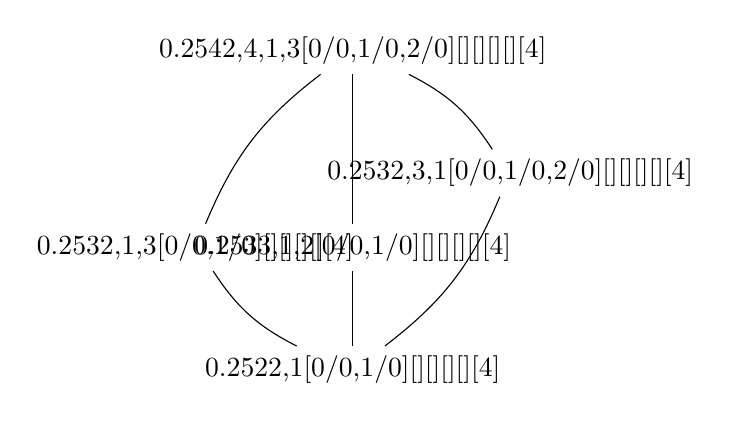
\begin{tikzpicture}
\def\y{1.35}
\def\x{2}
\def\s{0.25}
\node (2413) at (0*\x,3*\y){\patt{\s}{4}{2,4,1,3}[0/0,1/0,2/0][][][][][4]};
\node (213) at (-1*\x,1.15*\y){\patt{\s}{3}{2,1,3}[0/0,1/0][][][][][4]};
\node (312) at (0*\x,1.15*\y){\patt{\s}{3}{3,1,2}[0/0,1/0][][][][][4]};
\node (231) at (1*\x,1.85*\y){\patt{\s}{3}{2,3,1}[0/0,1/0,2/0][][][][][4]};
\node (21) at (0*\x,0*\y){\patt{\s}{2}{2,1}[0/0,1/0][][][][][4]};
\draw[-] (21) to [bend left=15] (213);
\draw[-] (21) to (312);
\draw[-] (21) to [bend right=15] (231);
\draw[-] (213) to [bend left=15] (2413);
\draw[-] (312) to (2413);
\draw[-] (231) to [bend right=15] (2413);
\end{tikzpicture}
\caption{The interval $[21^{(0,0),(1,0)},2413^{(0,0),(1,0),(2,0)}]$,
 which is pure but contains both pure and impure edges.}
 \label{fig:pureIm}
\end{figure}

\section{Topology}\label{sec:topology}
A full classification of shellable intervals has not been obtained for the classical permutation
poset, so finding such a classification for the mesh pattern poset would be equally difficult, if not more so.
However, in \cite{McSt13} all disconnected intervals are described, and containing a disconnected subinterval
implies a pure interval is not shellable. So this gives a large class of non-shellable intervals, in fact
it is shown that almost all intervals are not shellable. By \cref{lem:strongdis} containing a strongly
disconnected interval implies a non-pure interval is not shellable. So in this section we consider
which intervals contain such intervals. Firstly we look at the relationship between connectivity
in $\mathcal{P}$ and $\mathcal{M}$.

The connectivity of the interval $[\cl{m},\cl{p}]$ in $\mathcal{P}$ does
not necessarily imply the same property for $[m,p]$ in $\mathcal{M}$.
For example, the interval $[123,456123]$ is disconnected in $\mathcal{P}$ but the
interval $$[a,b]=[123^{(3,0),(3,1),(3,2)},456123^{(6,0),(6,1),(6,2)}],$$ see
\cref{fig:123}, is a chain in $\mathcal{M}$, so is connected. Furthermore, the interval
$[321,521643]$ is connected in $\mathcal{P}$ but the interval
$$[x,y]=[321^{(1, 3)},521643^{(1, 5),(1, 6), (4, 6)}],$$ see \cref{fig:321}, is strongly
disconnected in~$\mathcal{M}$.

The above examples imply that if $[\cl{m},\cl{p}]$ is (non-)shellable in $\mathcal{P}$
then it is not true that $[m,p]$ has the same property in $\mathcal{M}$. For example,
$[123,456123]$ is not shellable but $[a,b]$ is shellable, and
$[321,521643]$ is shellable but $[x,y]$
is not shellable.

\begin{figure}[h]\centering
\begin{subfigure}{0.45\textwidth}\centering
\patt{.25}{3}{1,2,3}[3/0,3/1,3/2][][][][][4]
\patt{.25}{6}{4,5,6,1,2,3}[6/0,6/1,6/2][][][][][4]
\caption{$123^{(3,0),(3,1),(3,2)}$ and $456123^{(6,0),(6,1),(6,2)}$}\label{fig:123}
\end{subfigure}
\begin{subfigure}{0.45\textwidth}\centering
\patt{.25}{3}{3,2,1}[1/3][][][][][4]
\patt{.25}{6}{5,2,1,6,4,3}[1/5,1/6,4/6][][][][][4]
\caption{$321^{(1, 3)}$ and $521643^{(1, 5), (1, 6), (4, 6)}$}\label{fig:321}
\end{subfigure}
\caption{}
\end{figure}

In \cite{McSt13} to show that almost all intervals are not shellable in $\mathcal{P}$
the direct sum operation is used. We can generalise the direct sum operation to
mesh patterns. Given two permutations $\alpha=\alpha_1\ldots\alpha_a$ and
$\beta=\beta_1\ldots\beta_b$ the direct sum of the two is defined as
$\alpha\oplus\beta=\alpha_1\ldots\alpha_a(\beta_1+a)(\beta_2+a)\ldots(\beta_b+a)$,
that is, we append $\beta$ to $\alpha$ and increase the value of each letter by the
length of $\alpha$. This can also be thought of in terms of the plots of $\alpha$
and $\beta$ by placing a copy of $\beta$ to the north east of $\alpha$.
Similarly we can define the skew-sum $\alpha\ominus\beta$ by
prepending $\alpha$ to $\beta$ and increasing the value of each letter of $\alpha$
by the length of $\beta$. We extend these definition to mesh patterns in the following way:

\begin{defn}\label{defn:directsum}
Consider two mesh patterns $s$ and $t$, where the top right corner of $s$
and bottom left corner of $t$ are not shaded. The direct sum $s\oplus t$ has classical pattern
$\cl{s}\oplus\cl{t}$ and shade the boxes $\sh{s}\cup\{(i,j+|\cl{s}|)\,|\,(i,j)\in\sh{t}\}$,
and also for any shaded boxes $(i,|\cl{s}|)$, $(|\cl{s}|,i)$, $(j,|\cl{s}|)$ or $(j,|\cl{s}|)$,
shaded all the boxes north, east, south or east of the box, respectively,
for all $0\le i< |\cl{s}|$ and $|\cl{s}|< j< |\cl{s}|+|\cl{t}|$.  We similarly
define the skew-sum for when the bottom right corner of $s$ and top left corner of $t$ are not shaded.
\end{defn}

The direct product $s\oplus t$ can be consider as placing a copy of $t$
north east of $s$ and any shaded box that was on a boundary we extend to the new boundary,
see \cref{fig:directsum}. We define the direct sum in this way because it maintains one of the most
important properties in the permutation sense, that the first $|\cl{s}|$ letters are
an occurrence of $s$ and the final $|\cl{t}|$ letters are an occurrence of $t$.

A permutation is said to be indecomposable if it cannot be written as the direct
sum of smaller permutation. We can generalise this to mesh patterns.
\begin{defn}
We say a mesh pattern $m$ is \emph{indecomposable} (resp. \emph{skew-indecomposable}) if it
cannot be written $m=a\oplus b$ (resp. $m=a\ominus b$), for some pair $a,b\not=m$.
\end{defn}
\begin{rem}
It is well known that a permutation has a unique decomposition into indecomposable permutation.
Which implies that a mesh pattern also has a unique decomposition.
\end{rem}

Using these definitions we can give a large class of strongly disconnected intervals,
which is a mesh pattern generalisation of Lemma 4.2 in \cite{McSt13}.

\begin{figure}\centering
$\patt{.5}{3}{1,3,2}[1/3,2/2]\oplus\patt{.5}{3}{3,2,1}[0/3,1/2,2/1,3/3,3/0][][][][][4]
=\patt{.5}{6}{1,3,2,6,5,4}[1/3,2/2,3/6,4/5,5/4,6/6,6/3,1/4,1/5,1/6,0/6,2/6,6/0,6/1,6/2][][][][][4]$
\caption{The direct sum of two mesh patterns.}\label{fig:directsum}
\end{figure}

\begin{lem}
If $m$ is indecomposable, $\dim m > 1$ and $(0,0),(|m|,|m|)\not\in\sh{m}$, then
$[m,m\oplus m]$ is strongly disconnected.
\begin{proof}
By Lemma 4.2 in \cite{McSt13} the interval $[\cl{m},\cl{m\oplus m}]$ is strongly disconnected,
with components $P_1=\{\cl{m}\oplus x\,|\,x\in [1,\cl{m})\}$ and
$P_2=\{x\oplus \cl{m}\,|\,x\in [1,\cl{m})\}$. So take any pair $\alpha,\beta\in[m,m\oplus m]$
if $\cl{\alpha}$ and $\cl{\beta}$ are not in the same component of  $[\cl{m},\cl{m\oplus m}]$,
then $\alpha$ and $\beta$ are incomparable. Let $\hat{P_1}=\{\alpha\,|\,\cl{\alpha}\in P_1\}$
and $\hat{P_2}=\{\alpha\,|\,\cl{\alpha}\in P_2\}$. However, $\hat{P_1}\cup\hat{P_2}\not=(\cl{m},\cl{m\oplus m})$
because it does not include the mesh patterns with $\cl{\alpha}=\cl{m\oplus m}$.

There are exactly two occurrences of $m$ in $m\oplus m$. These are $\eta_1$ the first $|m|$ letters
and $\eta_2$ the last $|m|$ letters. Note that each shaded box of $m\oplus m$ is used by at least one
of $\eta_1$ and $\eta_2$, so if we deshade a box the resulting pattern $x$ contains at most one occurrence of $m$,
either the first or last $|m|$ letters. Let $Q_1$ and $Q_2$ be sets of patterns with underlying permutation
$\cl{m\oplus m}$ where the first and last $|m|$ letters are the only occurrence of $m$, respectively. So any
element $Q_1$ cannot contain any element in $P_2\cup Q_2$ and similarly any element of $Q_2$ cannot
contain an element of $P_1\cup Q_1$. Therefore, $P_1\cup Q_1$ and $P_2\cup Q_2$ are disconnected components of
$[m,m\oplus m]$.
\end{proof}
\end{lem}
\begin{cor}
If $m$ is skew-indecomposable, $\dim m>1$ and $(|m|,0),(0,|m|)\not\in\sh{m}$, then
$[m,m\ominus m]$ is strongly disconnected.
\end{cor}

Using Lemma 4.2 in \cite{McSt13} it is shown that
almost all intervals of the classical permutation poset are not shellable. The
proof of this follows from the Marcus-Tardos theorem, we have seen this result
does not apply in the mesh pattern case so we cannot prove a similar result
using this technique.  A similar problem was studied for boxed mesh patterns in
permutations in \cite{AKV13}, which is equivalent to boxed mesh patterns in
fully shaded mesh patterns. So we leave it as an open question:

\begin{que}
What proportion of intervals of $\mathcal{M}$ are shellable?
\end{que}

\section{Open Questions}
It was conjectured in \cite{McSt13} that every interval of the classical permutation poset is unimodal.
 We conjecture that the same property is true of the mesh pattern poset.
\begin{conj}
Every interval of $\mathcal{M}$ is unimodal.
\end{conj}

The M\"obius function in the permutation poset can be computed more easily by decomposing the
permutations into smaller parts using the direct sum, or skew-sum, see \cite{BJJS11,McSt13}. Can a similar
result be obtained for mesh patterns?

\bibliographystyle{alpha}
\bibliography{bibfile}
\end{document}
